\subsection{Butterfly} \label{subsec:butterfly}

\subsubsection*{Allgemein}

Der Butterfly Algorithmus ist ein interpolierender Unterteilungsalgorithmus,
der von Nira Dyn, David Levine und John A. Gregory entwickelt wurde.
Butterfly arbeitet auf Dreiecksnetzen und erzeugt an regulären Stellen
\(C^1\) stetige Flächen, an extraordinären Stellen
(Valenz gleich drei oder größer sieben) jedoch lediglich \(C^0\).
\cite[S. 64ff]{Standford.24.07.2015} \cite[S. 72ff]{Zorin.subdivcourse}
\cite{Seeger01asub-atomic}
\cite{Gamasutra}
\cite{Sharp}
\cite{Zorin:1996:ISM:237170.237254}

\subsubsection*{Unterteilungs- und Randregeln}

Der Algorithmus besteht aus zwei Schritten:
\begin{enumerate}
\item Berechne für jede Kante einen Edge Point.
\item Ersetze jedes Dreieck durch vier neue Dreiecke.
\end{enumerate}

\begin{figure}
\centering
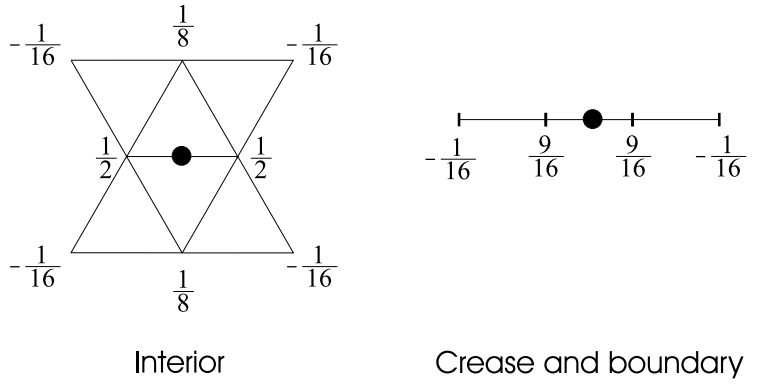
\includegraphics[width=0.8\textwidth]{content/media/sd_butterfly_mask.jpg}
\caption{Butterfly Eight-Point Stencil und Randregel \cite{Seeger01asub-atomic}}
\label{fig:sd_butterfly_mask}
\end{figure}

\paragraph*{Edge Point}
Die Berechnung des Edge Points wird mit dem sogenannten Eight-Point Stencil
aus \autoref{fig:sd_butterfly_mask} durchgeführt.
Die Regel für den Randfall ist daneben abgebildet.


Da die Punkte beim Butterfly interpoliert werden, müssen die alten Vertices
(wie bisher bei approximierenden Algorithmen) nicht neu berechnet werden. 

\paragraph*{Face Split}
Der Face Split ist identisch zum Loop Face Split.
Jedes Dreieck wird in vier neue Dreiecke aufgeteilt (\autoref{fig:sd_loop_split}).
\cite[S. 64ff]{Standford.24.07.2015} \cite[S. 72ff]{Zorin.subdivcourse}
\cite{Seeger01asub-atomic}
\cite{Gamasutra}
\cite{Sharp}
\cite{Zorin:1996:ISM:237170.237254}